\begin{center}
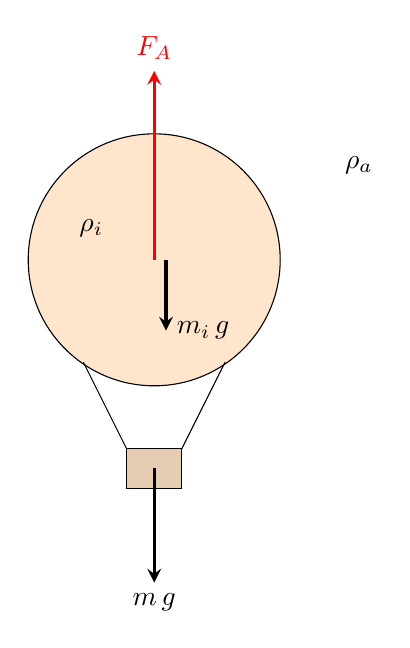
\begin{tikzpicture}[>=stealth]
 \draw[fill=orange!20] (0,2.2) circle (1.6);
 \draw (-0.9,0.9) -- (-0.35,-0.2);
 \draw (0.9,0.9) -- (0.35,-0.2);
 \draw[fill=brown!40] (-0.35,-0.2) rectangle (0.35,-0.7);
 \draw[->, very thick, red] (0,2.2) -- (0,4.6) node[above] {$F_\text{A}$};
 \draw[->, very thick] (0.15,2.2) -- (0.15,1.3) node[right] {$m_\text{i}\,g$};
 \draw[->, very thick] (0,-0.45) -- (0,-1.9) node[below] {$m\,g$};
 \node at (-0.8,2.6) {$\rho_\text{i}$};
 \node at (2.6,3.4) {$\rho_\text{a}$};
\end{tikzpicture}
\end{center}

\begin{abcliste}
\abc Das Volumen der Hülle ist
\begin{align}
 V &= \VBF = \frac{4}{3}\pi\cdot\left(\rB\right)^3 = \VB
\end{align}
Der Auftrieb ist die Gewichtskraft der verdrängten Aussenluft:
\begin{align}
 F_\text{A} &= \FABF \\
   &= \rhoLa\cdot\gE\cdot\VB \\
   &= \FAB \approx \result{\FABP{3}{2}}
\end{align}

\abc Der Ballon schwebt, wenn der Auftrieb die Last $m$ und die heisse Luft in der Hülle (Masse $m_\text{i} = \rho_\text{i}\,V$) trägt:
\begin{align}
 \rho_\text{a}\,V\,g &= \left(m + \rho_\text{i}\,V\right)g
\end{align}
Aufgelöst nach der Dichte der Innenluft:
\begin{align}
 \rho_\text{i} &= \rhoiF \\
   &= \rhoLa - \frac{\mLa}{\VB} \\
   &= \rhoi \approx \result{\rhoiP{0}{2}}
\end{align}
\end{abcliste}
